% Options for packages loaded elsewhere
\PassOptionsToPackage{unicode}{hyperref}
\PassOptionsToPackage{hyphens}{url}
\PassOptionsToPackage{dvipsnames,svgnames,x11names}{xcolor}
%
\documentclass[
  letterpaper,
  DIV=11,
  numbers=noendperiod]{scrartcl}

\usepackage{amsmath,amssymb}
\usepackage{iftex}
\ifPDFTeX
  \usepackage[T1]{fontenc}
  \usepackage[utf8]{inputenc}
  \usepackage{textcomp} % provide euro and other symbols
\else % if luatex or xetex
  \usepackage{unicode-math}
  \defaultfontfeatures{Scale=MatchLowercase}
  \defaultfontfeatures[\rmfamily]{Ligatures=TeX,Scale=1}
\fi
\usepackage[]{libertinus}
\ifPDFTeX\else  
    % xetex/luatex font selection
\fi
% Use upquote if available, for straight quotes in verbatim environments
\IfFileExists{upquote.sty}{\usepackage{upquote}}{}
\IfFileExists{microtype.sty}{% use microtype if available
  \usepackage[]{microtype}
  \UseMicrotypeSet[protrusion]{basicmath} % disable protrusion for tt fonts
}{}
\makeatletter
\@ifundefined{KOMAClassName}{% if non-KOMA class
  \IfFileExists{parskip.sty}{%
    \usepackage{parskip}
  }{% else
    \setlength{\parindent}{0pt}
    \setlength{\parskip}{6pt plus 2pt minus 1pt}}
}{% if KOMA class
  \KOMAoptions{parskip=half}}
\makeatother
\usepackage{xcolor}
\setlength{\emergencystretch}{3em} % prevent overfull lines
\setcounter{secnumdepth}{-\maxdimen} % remove section numbering
% Make \paragraph and \subparagraph free-standing
\ifx\paragraph\undefined\else
  \let\oldparagraph\paragraph
  \renewcommand{\paragraph}[1]{\oldparagraph{#1}\mbox{}}
\fi
\ifx\subparagraph\undefined\else
  \let\oldsubparagraph\subparagraph
  \renewcommand{\subparagraph}[1]{\oldsubparagraph{#1}\mbox{}}
\fi


\providecommand{\tightlist}{%
  \setlength{\itemsep}{0pt}\setlength{\parskip}{0pt}}\usepackage{longtable,booktabs,array}
\usepackage{calc} % for calculating minipage widths
% Correct order of tables after \paragraph or \subparagraph
\usepackage{etoolbox}
\makeatletter
\patchcmd\longtable{\par}{\if@noskipsec\mbox{}\fi\par}{}{}
\makeatother
% Allow footnotes in longtable head/foot
\IfFileExists{footnotehyper.sty}{\usepackage{footnotehyper}}{\usepackage{footnote}}
\makesavenoteenv{longtable}
\usepackage{graphicx}
\makeatletter
\def\maxwidth{\ifdim\Gin@nat@width>\linewidth\linewidth\else\Gin@nat@width\fi}
\def\maxheight{\ifdim\Gin@nat@height>\textheight\textheight\else\Gin@nat@height\fi}
\makeatother
% Scale images if necessary, so that they will not overflow the page
% margins by default, and it is still possible to overwrite the defaults
% using explicit options in \includegraphics[width, height, ...]{}
\setkeys{Gin}{width=\maxwidth,height=\maxheight,keepaspectratio}
% Set default figure placement to htbp
\makeatletter
\def\fps@figure{htbp}
\makeatother
\newlength{\cslhangindent}
\setlength{\cslhangindent}{1.5em}
\newlength{\csllabelwidth}
\setlength{\csllabelwidth}{3em}
\newlength{\cslentryspacingunit} % times entry-spacing
\setlength{\cslentryspacingunit}{\parskip}
\newenvironment{CSLReferences}[2] % #1 hanging-ident, #2 entry spacing
 {% don't indent paragraphs
  \setlength{\parindent}{0pt}
  % turn on hanging indent if param 1 is 1
  \ifodd #1
  \let\oldpar\par
  \def\par{\hangindent=\cslhangindent\oldpar}
  \fi
  % set entry spacing
  \setlength{\parskip}{#2\cslentryspacingunit}
 }%
 {}
\usepackage{calc}
\newcommand{\CSLBlock}[1]{#1\hfill\break}
\newcommand{\CSLLeftMargin}[1]{\parbox[t]{\csllabelwidth}{#1}}
\newcommand{\CSLRightInline}[1]{\parbox[t]{\linewidth - \csllabelwidth}{#1}\break}
\newcommand{\CSLIndent}[1]{\hspace{\cslhangindent}#1}

\usepackage{booktabs}
\usepackage{longtable}
\usepackage{array}
\usepackage{multirow}
\usepackage{wrapfig}
\usepackage{float}
\usepackage{colortbl}
\usepackage{pdflscape}
\usepackage{tabu}
\usepackage{threeparttable}
\usepackage{threeparttablex}
\usepackage[normalem]{ulem}
\usepackage{makecell}
\usepackage{xcolor}
\KOMAoption{captions}{tableheading}
\makeatletter
\makeatother
\makeatletter
\makeatother
\makeatletter
\@ifpackageloaded{caption}{}{\usepackage{caption}}
\AtBeginDocument{%
\ifdefined\contentsname
  \renewcommand*\contentsname{Table of contents}
\else
  \newcommand\contentsname{Table of contents}
\fi
\ifdefined\listfigurename
  \renewcommand*\listfigurename{List of Figures}
\else
  \newcommand\listfigurename{List of Figures}
\fi
\ifdefined\listtablename
  \renewcommand*\listtablename{List of Tables}
\else
  \newcommand\listtablename{List of Tables}
\fi
\ifdefined\figurename
  \renewcommand*\figurename{Figure}
\else
  \newcommand\figurename{Figure}
\fi
\ifdefined\tablename
  \renewcommand*\tablename{Table}
\else
  \newcommand\tablename{Table}
\fi
}
\@ifpackageloaded{float}{}{\usepackage{float}}
\floatstyle{ruled}
\@ifundefined{c@chapter}{\newfloat{codelisting}{h}{lop}}{\newfloat{codelisting}{h}{lop}[chapter]}
\floatname{codelisting}{Listing}
\newcommand*\listoflistings{\listof{codelisting}{List of Listings}}
\makeatother
\makeatletter
\@ifpackageloaded{caption}{}{\usepackage{caption}}
\@ifpackageloaded{subcaption}{}{\usepackage{subcaption}}
\makeatother
\makeatletter
\@ifpackageloaded{tcolorbox}{}{\usepackage[skins,breakable]{tcolorbox}}
\makeatother
\makeatletter
\@ifundefined{shadecolor}{\definecolor{shadecolor}{rgb}{.97, .97, .97}}
\makeatother
\makeatletter
\makeatother
\makeatletter
\makeatother
\ifLuaTeX
  \usepackage{selnolig}  % disable illegal ligatures
\fi
\IfFileExists{bookmark.sty}{\usepackage{bookmark}}{\usepackage{hyperref}}
\IfFileExists{xurl.sty}{\usepackage{xurl}}{} % add URL line breaks if available
\urlstyle{same} % disable monospaced font for URLs
\hypersetup{
  pdftitle={Causal effects of religious de-identification on multi-dimensional well-being},
  pdfauthor={Joseph A. Bulbulia; Don E Davis; Ken Rice; Geoffrey Troughton; Daryl Van Tongeren; Chris G. Sibley},
  pdfkeywords={Author order TBA.},
  colorlinks=true,
  linkcolor={blue},
  filecolor={Maroon},
  citecolor={Blue},
  urlcolor={Blue},
  pdfcreator={LaTeX via pandoc}}

\title{Causal effects of religious de-identification on
multi-dimensional well-being}
\usepackage{etoolbox}
\makeatletter
\providecommand{\subtitle}[1]{% add subtitle to \maketitle
  \apptocmd{\@title}{\par {\large #1 \par}}{}{}
}
\makeatother
\subtitle{An outcome-wide study}
\author{Joseph A. Bulbulia \and Don E Davis \and Ken Rice \and Geoffrey
Troughton \and Daryl Van Tongeren \and Chris G. Sibley}
\date{}

\begin{document}
\maketitle
\begin{abstract}
Max Weber described the loss of religion as ``the disenchantment of the
world.'' However, quantifying the mangitude of disenchantment from the
loss of religion has yet to be attempted. Indeed, whether religious
disaffiliation causally affects people at all is unclear and cannot be
determined from cross-sectional data. Here, we use a potential outcomes
framework from causal inference to contrast the expected effects of
religious disaffilation accross a wide range of multi-dimensional
wellbeing, one year after religious change.
\end{abstract}
\ifdefined\Shaded\renewenvironment{Shaded}{\begin{tcolorbox}[interior hidden, frame hidden, borderline west={3pt}{0pt}{shadecolor}, breakable, enhanced, boxrule=0pt, sharp corners]}{\end{tcolorbox}}\fi

\hypertarget{introduction}{%
\subsection{Introduction}\label{introduction}}

Max Weber famously described the loss of religion as ``the
disenchantment of the world'' (Wilson, J., and Sibley 2014). However, it
is unclear whether, and in which ways, disaffiliation causes
disenchantment.

Although cross-sectional data may be suggestive of relationships,
cross-sectional data are essentially useless for inferring causality.
For example, it is possible that people who score low in meaning of life
tend to shed their religious affiliation at a higher rate than people
who score high in meaning of life. The associations in cross-sectional
data cannot rule out this possibility. It is plausible that individuals
with low life meaning are more likely to distance themselves from
religious institutions, leading to an over-representation of
disenchantment among non-religious individuals in cross-sectional
surveys. If we were to intervene to make the disenchanted re-affiliate
this might lead to greater loss of meaning.

Here, we use longitudinal data to emulate an idealised experiment, thus
providing a clearer window into the direction of causality (Hernán et
al. 2016; Bulbulia 2022; Hernan and Robins 2023)

\hypertarget{sample}{%
\subsubsection{Sample}\label{sample}}

\hypertarget{eligibility-criteria}{%
\subsubsection{Eligibility criteria}\label{eligibility-criteria}}

To emulate randomisation with observational data, we selected (1) those
participants who were identified as religious at the baseline wave
(NZAVS wave 2018) and who (2) reported a religious identification one
year later. There were 12,600 participants who met these criteria.

\hypertarget{disaffiation-rates}{%
\subsubsection{Disaffiation rates}\label{disaffiation-rates}}

As indicated in Table~\ref{tbl-transition}, of the 12600 people who were
religious at baseline, 1977 people dis-affiliated participants one year
later (NZAVS wave 2019), at the measurement year.\footnote{Cite our
  Markov paper showing that much religious change is probably
  artifactual.}

\hypertarget{tbl-transition}{}
\begin{longtable}[]{@{}ccc@{}}
\caption{\label{tbl-transition}Transition matrix}\tabularnewline
\toprule\noalign{}
From & religious yes & religious not \\
\midrule\noalign{}
\endfirsthead
\toprule\noalign{}
From & religious yes & religious not \\
\midrule\noalign{}
\endhead
\bottomrule\noalign{}
\endlastfoot
religious yes & 10623 & 1977 \\
\end{longtable}

\hypertarget{assumptions-for-causal-inference}{%
\subsubsection{Assumptions for causal
inference}\label{assumptions-for-causal-inference}}

To assess a causal effect we must contrast how the world would turn out
if we were to intervene. Generally, we cannot observe individual causal
effects because for any individual case, we only observe the
intervention or its absence. We cannot both intervene and not-intervene
at once. This is called the fundamental problem of causal inference
(Bulbulia 2022). Although we cannot generally observe unit-level causal
effects, it may be possible to estimate average causal effects. We do
this by contrasting the average effect in the exposed group with the
average effect in the unexposed unexposed group. For example, average of
the contrast (or equivalently the contrast of the the
averages)\footnote{Note that mathematically, the difference in the
  average expectation is equivalent to the average of the differences in
  expectation.} on the difference scale may be expressed:

\begin{alignat*}{2}
ATE & = E[Y(1)) - E(Y(0)]\\
& = E=[Y(1) - Y(0)]
\end{alignat*}

Estimating the average treatment effects (ATE) of binary exposures or
contrasts between different exposure levels involves understanding
causal inference as counterfactual data science. The ATE is expressed
as:

   \begin{align*}
    ATE = E[Y(a) - Y(a*)]
    \end{align*}

Our causal inference is grounded on three critical assumptions:

\hypertarget{identification-assumption-1-causal-consistency}{%
\paragraph{Identification assumption 1: Causal
consistency}\label{identification-assumption-1-causal-consistency}}

Causal consistency assumes the observed outcome aligns with the
potential outcome for a given exposure level:

\[Y^{observed} = AY(a=1) + (1-A)Y(a=0)\]

Observed outcomes can represent counterfactual outcomes under certain
exposures, such that:

\[
Y^{observed}_i = 
\begin{cases} 
Y_i(~a^*) & \text{if } A_i = a* \\
Y_i(~a~) & \text{if } A_i = a
\end{cases}
\]

Causal consistency also assumes no interference between unit treatments,
allowing potential outcomes to be set to the observed outcomes. For this
assumption to hold, we require ``treatment variation irrelevance.'' If
there are (1) well-defined outcomes for each treatment version, and (2)
no confounding effects, the multiple versions of treatments can be used
to estimate the causal effect:

\[K \coprod Y(k) | L\] or equivalently \[Y(k) \coprod K | L\]

Here, the treatement \(A\) is essentially a function of \(K\)
treatments, \(A = f(k_1...k_v)\) versions

Limitations exist, however, when interventions are ill-defined, or the
causal effect's interpretation is ambiguous. Put simply, given there are
unknown ways of becoming religiously disaffiliated the interpretation of
``disaffiliation'' may be strained. It is strained in the sense that we
would not know how to intervene to \emph{make} a religiously affiliated
person disaffiliate. We will return to this question in the discussion.

\hypertarget{identification-assumption-2-exchangability}{%
\paragraph{Identification assumption 2:
Exchangability}\label{identification-assumption-2-exchangability}}

Exchangability assumes treatment assignment is independent of potential
outcomes, given observed covariates. This is the ``no-confounding''
assumption that many psychologists have learned in association with
experimental design. In the setting of obervational data, we emulate
randomisation by conditioning on indicators that may lead to an
association of the exposure \(A\) and the outcome \(Y\) in the absence
of causation.

\[Y(a)\coprod  A|L\] or \[A \coprod  Y(a)|L\]

Where exchangability holds, we calculate the Average Treatment Effect
(ATE)

\[
ATE = E[Y(a*)|L = l] - E[Y(a)|L = l] 
\]

Put differently, conditioning on confounders ensures \emph{balance} in
their distribution across exposures.

\hypertarget{identification-assumption-3-positivity}{%
\paragraph{Identification assumption 3:
Positivity}\label{identification-assumption-3-positivity}}

Positivity is satisfied if there's a positive probability of receiving
or not receiving exposure at all covariate levels. Expressed as:

\begin{equation}
0 < \Pr(A=a|L)<1, ~ \forall a \in A, ~ \forall a \in L
\end{equation}

There are two types of positivity violation.

\begin{itemize}
\item
  \textbf{Random non-positivity}: Occurs when the causal effect of a
  missing observation is presumed to exist. This violation is the only
  one verifiable by data. Here, we check and report it.
\item
  \textbf{Deterministic non-positivity}: Occurs when the causal effect
  is inconceivable. For example, the causal effect of hysterectomy in
  biological males violates deterministic non-positivity.
\end{itemize}

\hypertarget{identification-strategy}{%
\subsubsection{Identification Strategy}\label{identification-strategy}}

Effects must follow causes. To avoid the problems of reverse causation,
we measured outcomes during the year following the exposure (NZAVS wave
2020). We used doubly robust methods. These combine inverse probability
of treatment weights (propensity scores) with regression stratification.
There are two models at work in a doubly robust estimator.

\hypertarget{unconditional-doubly-robust-estimation-for-causal-effect-estimation}{%
\subsubsection{Unconditional Doubly Robust Estimation for Causal Effect
Estimation}\label{unconditional-doubly-robust-estimation-for-causal-effect-estimation}}

We use a Doubly Robust Estimation method, which effectively combines the
strengths of the IPTW and G-computation methods (see:
\href{https://go-bayes.github.io/psych-434-2023/content/09-content.html\#comprehensive-checklist-for-detailed-reporting-of-a-causal-inferenctial-study-e.g.-assessment-3-option-2}{here}.
The technique utilises both the propensity score and the outcome model,
making it ``doubly robust.'' This implies that if either of these models
is correctly specified, the estimation will not be biased.

\textbf{Step 1} The first step is to estimate the propensity score. The
propensity score, denoted as \(e(L)\), is the conditional probability of
the exposure \(A = 1\) given the covariates \(L\). The appropriate model
to estimate this can be chosen based on the nature of the data and the
exposure.

\[e = P(A = 1 | L) = f_A(L; \theta_A)\]

In this equation, \(f_A(L; \theta_A)\) is a function that estimates the
probability of the exposure \(A = 1\) given covariates \(L\). Here, we
use the \texttt{ebalance} method from the \texttt{clarify} package,
which we have found to ensure good balance on the confounders (see fig
below). We then calculate the weights for each individual, denoted as
\(v\), using the estimated propensity score:

\[
v = 
\begin{cases} 
\frac{1}{e} & \text{if } A = 1 \\
\frac{1}{1-e} & \text{if } A = 0 
\end{cases}
\]

Here, \(v\) depends on \(A\), and is calculated as the inverse of the
propensity score for exposed individuals and as the inverse of \(1-e\)
for unexposed individuals.

\textbf{Step 2} The next step involves fitting a weighted outcome model.
Using the weights computed from the estimated propensity scores, a model
for the outcome \(Y\), conditional on the exposure \(A\), is fitted.

\[ \hat{E}(Y|A, L; V) = f_Y(A, L ; \theta_Y, V) \]

In this model, \(f_Y\) is a function (in our case a weighted regression
model) with parameters \(θ_Y\). The weights \(V\) are incorporated into
the estimation process, affecting the contribution of each observation
to the estimation of \(θ_Y\), but they are not an additional variable in
the model. Additionally, following {``Agnostic Notes on Regression
Adjustments to Experimental Data: Reexamining Freedman{'}s Critique''}
(n.d.), we take the interaction of the exposure and baseline covariates
when estimating our regression model. For binary outcomes we model the
rate ratio using Poisson regression. Although binomial regression is
acceptable when the outcome is rare (less than 10\%), non-collapsability
leads means that we cannot interpret results as marginal causal effects.
For consistency we use the Poisson model with robust standard errors.

\textbf{Step 3} The third step is to simulate the potential outcome for
each individual under the hypothetical scenario where everyone is
exposed to the intervention \(A=a\), irrespective of their actual
exposure level:

\[\hat{E}(a) = \hat{E}[Y_i|A=a; L,\hat{\theta}_Y, v_i]\]

This expectation is calculated for each individual \(i\), with
individual-specific weights \(v_i\).

\textbf{Step 4} Finally, we estimate the average causal effect. We
compute the estimated expected value of the potential outcomes under
each intervention level:

\[\hat{\delta} = \hat{E}[Y(a)] - \hat{E}[Y(a')]\]

The difference \(\delta\) represents the average causal effect of
changing the exposure from level \(a'\) to level \(a\).

For standard errors and confidence intervals, we use simulation-based
inference methods (Greifer et al. 2023).

\hypertarget{baseline-confounders-exposure-and-outcome-measures}{%
\subsubsection{Baseline confounders, exposure, and outcome
measures}\label{baseline-confounders-exposure-and-outcome-measures}}

See Appendix 1

\hypertarget{results}{%
\subsection{Results}\label{results}}

\hypertarget{effects-on-health}{%
\subsubsection{Effects on health}\label{effects-on-health}}

Figure Figure~\ref{fig-results-health-propensity-scores} reveals strong
imbalance prior to propensity score estimation.

\begin{figure}

{\centering \includegraphics[width=1\textwidth,height=\textheight]{target-trial-religion-loss_files/figure-latex/fig-results-health-propensity-scores-1.pdf}

}

\caption{\label{fig-results-health-propensity-scores}Love plot for
propensity score analysis: Health outcomes.}

\end{figure}

As indicate in @ fig-results-health, the expected + one-year effect of
religious disaffiliation does not reliably affect health as subjectively
reported across NZAVS domains. However, we find that disaffilation is
causally associated with increases in both the average intensity and
frequency of alcohol consumption.

It has long been known that alcohol consumption can have damaging health
and social effects. However, it is unclear whether the changes we detect
here translate to other domains.

\begin{figure}

{\centering 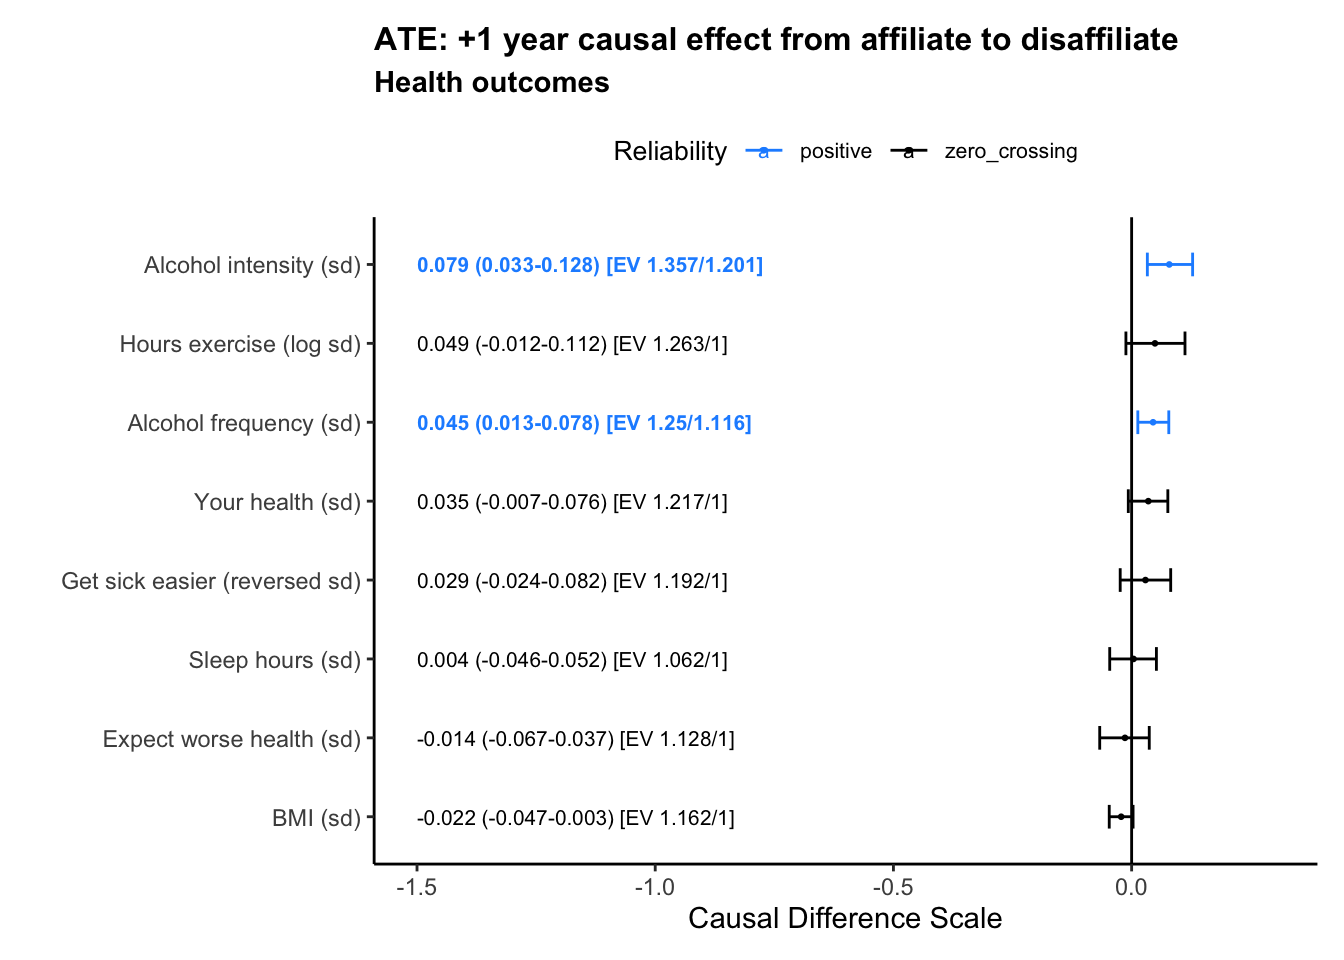
\includegraphics{target-trial-religion-loss_files/figure-latex/fig-results-health-1.pdf}

}

\caption{\label{fig-results-health}Causal effects of religious loss on
reported physical health}

\end{figure}

\begin{figure}

{\centering 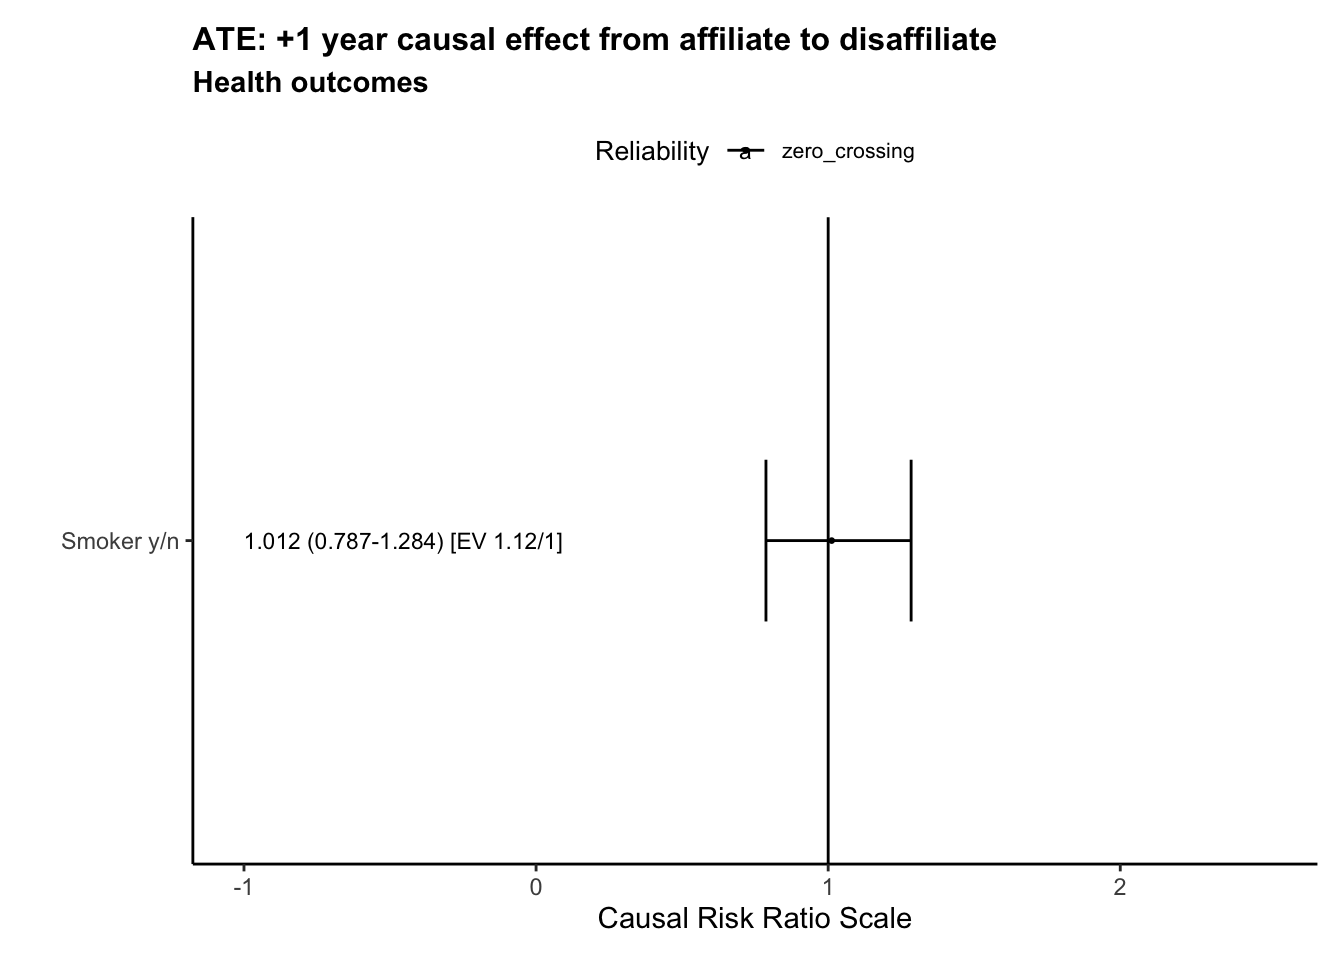
\includegraphics{target-trial-religion-loss_files/figure-latex/fig-results-health-rr-1.pdf}

}

\caption{\label{fig-results-health-rr}Causal effects of religious loss
on smoking (risk ratio)}

\end{figure}

\hypertarget{effects-on-embodied-well-being}{%
\subsubsection{Effects on embodied
well-being}\label{effects-on-embodied-well-being}}

\begin{figure}

{\centering 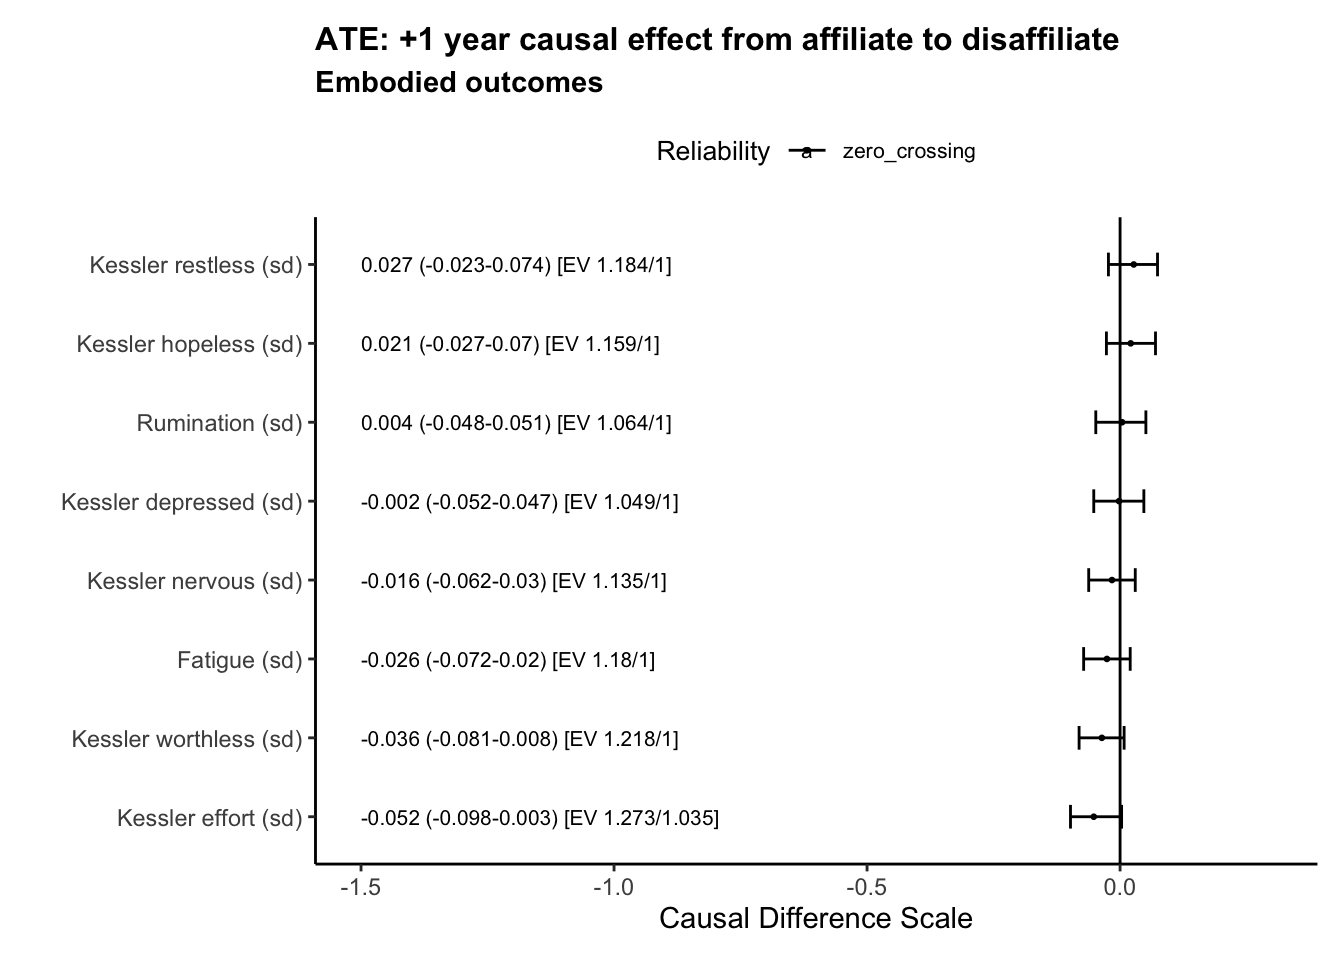
\includegraphics{target-trial-religion-loss_files/figure-latex/fig-results-embodied-1.pdf}

}

\caption{\label{fig-results-embodied}Causal effects of religious loss on
embodied well-being}

\end{figure}

\hypertarget{effects-on-practical-well-being}{%
\subsubsection{Effects on practical
well-being}\label{effects-on-practical-well-being}}

\begin{figure}

{\centering 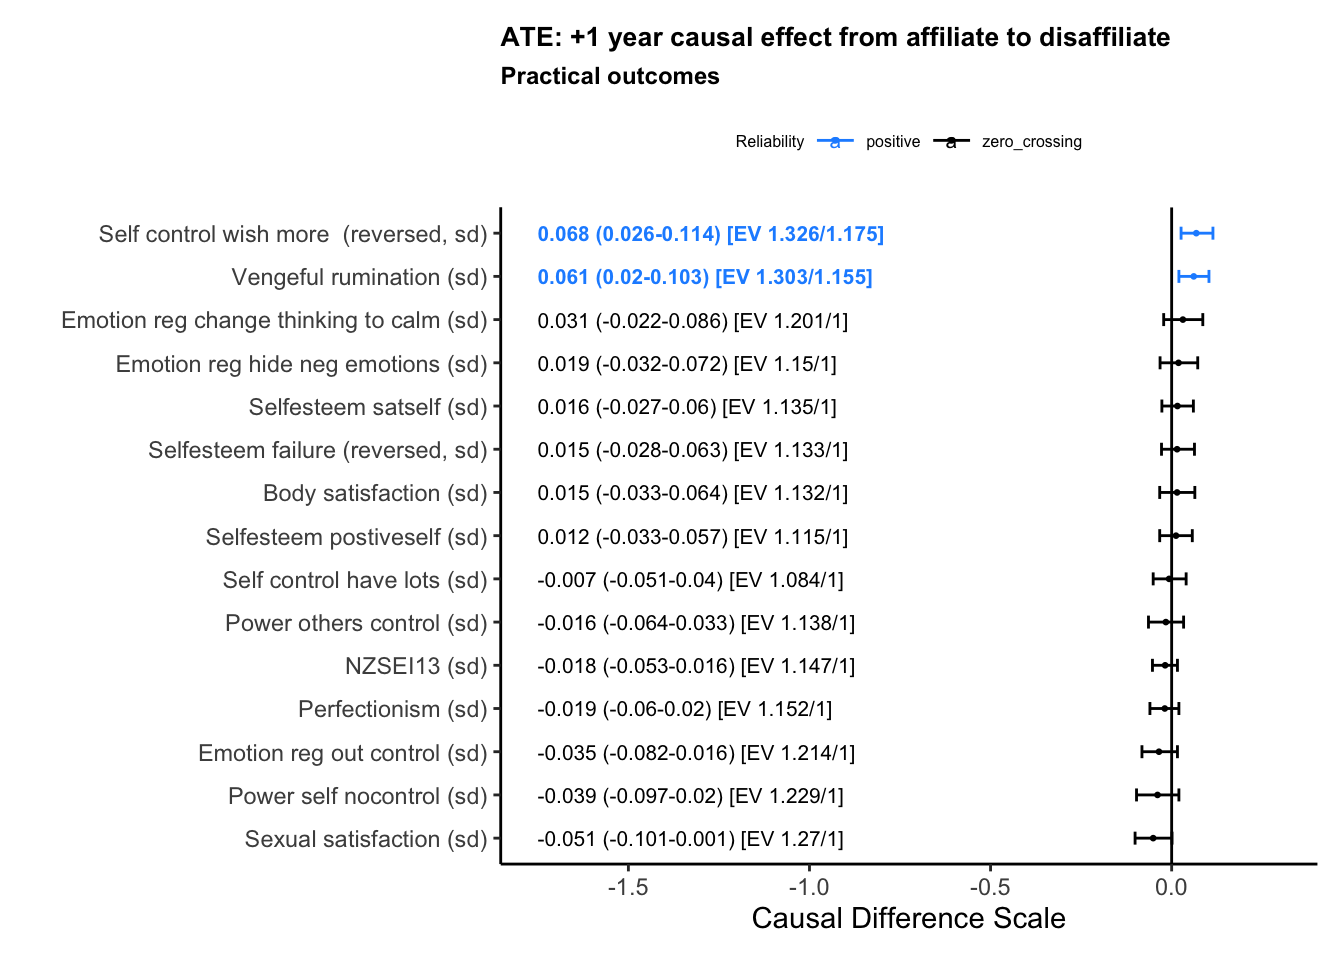
\includegraphics{target-trial-religion-loss_files/figure-latex/fig-results-practical-well-being-1.pdf}

}

\caption{\label{fig-results-practical-well-being}Causal effects of
religious loss on practical well-being}

\end{figure}

\hypertarget{effects-on-reflective-well-being}{%
\subsubsection{Effects on reflective
well-being}\label{effects-on-reflective-well-being}}

\begin{figure}

{\centering \includegraphics{target-trial-religion-loss_files/figure-latex/fig-results-reflective-well-being-1.pdf}

}

\caption{\label{fig-results-reflective-well-being}Causal effects of
religious loss on reflective well-being}

\end{figure}

\hypertarget{effects-social-well-being}{%
\subsubsection{Effects social
well-being}\label{effects-social-well-being}}

\begin{figure}

{\centering \includegraphics{target-trial-religion-loss_files/figure-latex/fig-results-social-well-being-1.pdf}

}

\caption{\label{fig-results-social-well-being}Causal effects of
religious loss on reflective well-being}

\end{figure}

\begin{figure}

{\centering 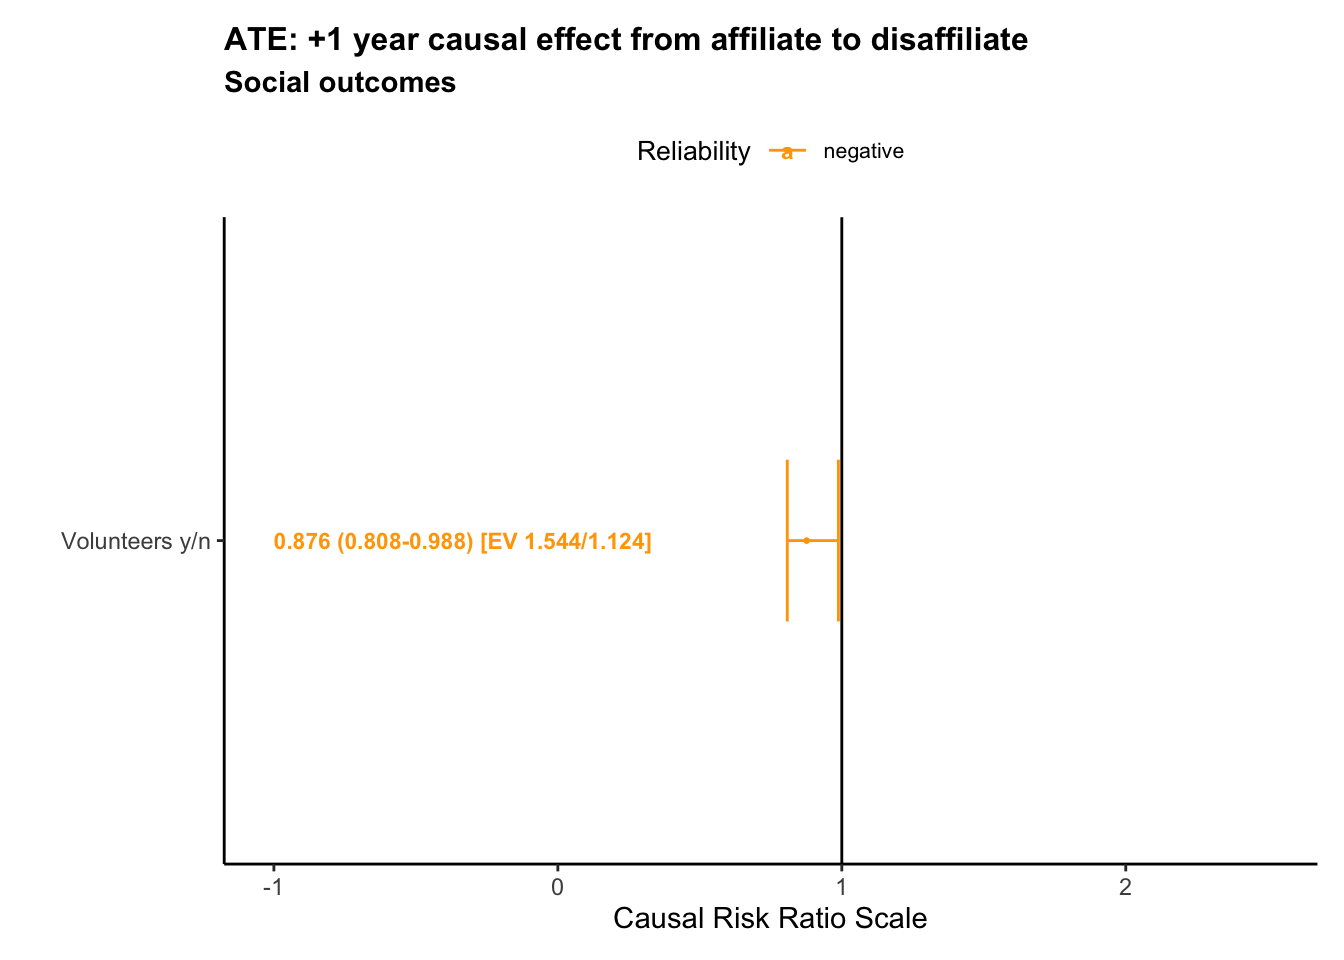
\includegraphics{target-trial-religion-loss_files/figure-latex/fig-models-social-risk-ratio-1.pdf}

}

\caption{\label{fig-models-social-risk-ratio}Causal effects of religious
loss on volunteering.}

\end{figure}

\hypertarget{discussion}{%
\subsection{Discussion}\label{discussion}}

Here, we combined rigorous methods from causal epidemiology with
national scale time-series data to estimate the causal effects of
religious disaffiliation on multidimensional well-being. We used doubly
robust methods that combine propensity score weights with regression
stratification. By controlling for measures of all outcomes at baseline
we reduce the probability of unmeasured confounding. Because this cannot
be ensured, we report E-values, a sensitivity analysis that clarifies
the ``worst case'' scenario for an unmeasured confounder to explain away
the results.

\textbf{Health domain}: The expected +1 year effect of religious
disaffiliation is to increase both the average intensity and frequency
of alcohol consumption. We do not find reliable results on other health
domains.

\textbf{Embodied well-being domains}: We do not find reliable evidence
for a +1 year effect of religious disaffiliation on embodied will being
(i.e.~distress, fatigue)

\textbf{Practical well-being}: The expected +1 year effect of religious
disaffiliation is to diminish wishes for more self control. That is
good. However the one-year effect of disaffiliation is to increase
vengeful rumination. That is not good.

\textbf{Reflective well-being}: The expected +1 year effect of religious
disaffiliation is increase life satisfaction. That is good. However the
one-year effect of disaffiliation is to decrease a sense of purpose in
life. That is not good.

\textbf{Social well-being-being}: Disaffiliation is expected to cause
reduction in charitable giving and volunteering (consistent {[}cite a
different study{]}). However we do not find that disaffiliation as such
reduces other aspects of social well-being.

\hypertarget{generalisability-and-transportability}{%
\subsubsection{Generalisability and
Transportability}\label{generalisability-and-transportability}}

\begin{itemize}
\tightlist
\item
  We can generalise to the religious population of New Zealand. Whether
  results transport elsewhere is unclear.
\end{itemize}

\hypertarget{assumptions-and-limitations}{%
\subsubsection{Assumptions and
Limitations}\label{assumptions-and-limitations}}

\begin{enumerate}
\def\labelenumi{\arabic{enumi}.}
\tightlist
\item
  Consistency\ldots{}
\item
  Positivity\ldots{}
\item
  Exhangeability\ldots{}
\end{enumerate}

Also

\begin{enumerate}
\def\labelenumi{\arabic{enumi}.}
\tightlist
\item
  Measurement of religious change -- Markov models show less
\item
  Measurement error
\item
  Loss to follow up attrition (requires modelling assumptions.)
\end{enumerate}

\hypertarget{theoretical-relevance}{%
\subsubsection{Theoretical Relevance}\label{theoretical-relevance}}

This study is important both for its methods and findings.

\begin{enumerate}
\def\labelenumi{\arabic{enumi}.}
\tightlist
\item
  The bar for causality in this study very high.
\item
  It would generally be unexpected that in a country such as New
  Zealand, which is a highly secular, a change in one's religious
  affiliation would induce measurable effects on people within only
  one-year.
\end{enumerate}

\hypertarget{future-research}{%
\subsubsection{Future Research}\label{future-research}}

\begin{enumerate}
\def\labelenumi{\arabic{enumi}.}
\tightlist
\item
  We did not compare religious disaffiliates to people who are secular.
  Loss of religion suggests a loss of charity. However, secular people
  might be less charitable still. Future research\ldots{}
\item
  Previous research shows differences in these comparison groups (Van
  Tongeren et al. 2020; Sibley and Bulbulia 2012).
\end{enumerate}

\hypertarget{real-world-implications}{%
\subsubsection{Real-world Implications}\label{real-world-implications}}

In practical terms, the real-world implications of the findings, are
\ldots{}

\newpage{}

\hypertarget{appendix-a.-measures}{%
\subsection{Appendix A. Measures}\label{appendix-a.-measures}}

\hypertarget{baseline-confounding-control}{%
\subsubsection{Baseline confounding
control}\label{baseline-confounding-control}}

\hypertarget{age-waves-1-15}{%
\paragraph{Age (waves: 1-15)}\label{age-waves-1-15}}

We asked participants' age in an open-ended question (``What is your
age?'' or ``What is your date of birth'').

\hypertarget{disability-waves-5-15}{%
\paragraph{Disability (waves: 5-15)}\label{disability-waves-5-15}}

We assessed disability with a one item indicator adapted from Verbrugge
(1997), that asks ``Do you have a health condition or disability that
limits you, and that has lasted for 6+ months?'' (1 = Yes, 0 = No).

\hypertarget{education-attainment-waves-1-4-15}{%
\paragraph{Education Attainment (waves: 1,
4-15)}\label{education-attainment-waves-1-4-15}}

Participants were asked ``What is your highest level of
qualification?''. We coded participans highest finished degree according
to the New Zealand Qualifications Authority. Ordinal-Rank 0-10 NZREG
codes (with overseas school quals coded as Level 3, and all other
ancillary categories coded as missing)
See:https://www.nzqa.govt.nz/assets/Studying-in-NZ/New-Zealand-Qualification-Framework/requirements-nzqf.pdf

\hypertarget{employment-waves-1-3-4-11}{%
\paragraph{Employment (waves: 1-3,
4-11)}\label{employment-waves-1-3-4-11}}

We asked participants ``Are you currently employed? (This includes
self-employed or casual work)''. * note: This question disappeared in
the updated NZAVS Technical documents (Data Dictionary).

\hypertarget{european-waves-1-15}{%
\paragraph{European (waves: 1-15)}\label{european-waves-1-15}}

Participants were asked ``Which ethnic group do you belong to (NZ census
question)?'' or ``Which ethnic group(s) do you belong to? (Open-ended)''
(wave: 3). Europeans were coded as 1, whereas other ethnicities were
coded as 0.

\hypertarget{ethnicity-waves-3}{%
\paragraph{Ethnicity (waves: 3)}\label{ethnicity-waves-3}}

Based on the New Zealand Cencus, we asked participants ``Which ethnic
group(s) do you belong to?''. The responses were: (1) New Zealand
European; (2) Māori; (3) Samoan; (4) Cook Island Māori; (5) Tongan; (6)
Niuean; (7) Chinese; (8) Indian; (9) Other such as DUTCH, JAPANESE,
TOKELAUAN. Please state:. We coded their answers into four groups:
Maori, Pacific, Asian, and Euro (except for Time 3, which used an
open-ended measure).

\hypertarget{gender-waves-1-15}{%
\paragraph{Gender (waves: 1-15)}\label{gender-waves-1-15}}

We asked participants' gender in an open-ended question: ``what is your
gender?'' or ``Are you male or female?'' (waves: 1-5). Female was coded
as 0, Male was coded as 1, and gender diverse coded as 3 (Fraser et al.
2020). (or 0.5 = neither female nor male)

\hypertarget{income-waves-1-3-4-15}{%
\paragraph{Income (waves: 1-3, 4-15)}\label{income-waves-1-3-4-15}}

Participants were asked ``Please estimate your total household income
(before tax) for the year XXXX''. To stablise this indicator, we first
took the natural log of the response + 1, and then centred and
standardised the log-transformed indicator.

\hypertarget{job-security-waves-1-34-79-15}{%
\paragraph{Job Security (waves:
1-3,4-7,9-15)}\label{job-security-waves-1-34-79-15}}

Participants indicated their feeling of job security by answering ``How
secure do you feel in your current job?'' on a scale from 1 (not secure)
to 7 (very secure).

\hypertarget{parent-waves-5-15}{%
\paragraph{Parent (waves: 5-15)}\label{parent-waves-5-15}}

Participants were asked ``If you are a parent, what is the birth date of
your eldest child?'' or ``If you are a parent, in which year was your
eldest child born?'' (waves: 10-15). Parents were coded as 1, while the
others were coded as 0.

\hypertarget{number-of-children-waves-1-3-4-15}{%
\paragraph{Number of Children (waves: 1-3,
4-15)}\label{number-of-children-waves-1-3-4-15}}

We measured number of children using one item from
(\textbf{bulbulia2015?}). We asked participants ``How many children have
you given birth to, fathered, or adopted. How many children have you
given birth to, fathered, or adopted?'' or ````How many children have
you given birth to, fathered, or adopted. How many children have you
given birth to, fathered, and/or parented?'' (waves: 12-15).

\hypertarget{political-orientation}{%
\paragraph{Political Orientation}\label{political-orientation}}

We measured participants' political orientation using a single item
adapted from Jost (2006).

``Please rate how politically liberal versus conservative you see
yourself as being.''

(1 = Extremely Liberal to 7 = Extremely Conservative)

\hypertarget{nzsei-13-waves-8-15}{%
\paragraph{NZSEI-13 (waves: 8-15)}\label{nzsei-13-waves-8-15}}

We assessed occupational prestige and status using the New Zealand
Socio-economic Index 13 (NZSEI-13) (Fahy, Lee, and Milne 2017). This
index uses the income, age, and education of a reference group, in this
case the 2013 New Zealand census, to calculate an score for each
occupational group. Scores range from 10 (Lowest) to 90 (Highest). This
list of index scores for occupational groups was used to assign each
participant a NZSEI-13 score based on their occupation.

Participants were asked ``If you are a parent, what is the birth date of
your eldest child?''.

\hypertarget{living-with-partner}{%
\paragraph{Living with Partner}\label{living-with-partner}}

Participants were asekd ``Do you live with your partner?'' (1 = Yes, 0 =
No).

\hypertarget{living-in-an-urban-area-waves-1-15}{%
\paragraph{Living in an Urban Area (waves:
1-15)}\label{living-in-an-urban-area-waves-1-15}}

We coded whether they are living in an urban or rural area (1 = Urban, 0
= Rural) based on the addresses provided.

We coded whether they are living in an urban or rural area (1 = Urban, 0
= Rural) based on the addresses provided.

\hypertarget{nz-deprivation-index-waves-1-15}{%
\paragraph{NZ Deprivation Index (waves:
1-15)}\label{nz-deprivation-index-waves-1-15}}

We used the NZ Deprivation Index to assign each participant a score
based on where they live (Atkinson, Salmond, and Crampton 2019). This
score combines data such as income, home ownership, employment,
qualifications, family structure, housing, and access to transport and
communication for an area into one deprivation score.

\hypertarget{nz-born-waves-1-24-15}{%
\paragraph{NZ-Born (waves: 1-2,4-15)}\label{nz-born-waves-1-24-15}}

We asked participants ``Which country were you born in?'' or ``Where
were you born? (please be specific, e.g., which town/city?)'' (waves:
6-15).

\hypertarget{mini-ipip-6-waves-1-34-15}{%
\paragraph{Mini-IPIP 6 (waves:
1-3,4-15)}\label{mini-ipip-6-waves-1-34-15}}

We measured participants personality with the Mini International
Personality Item Pool 6 (Mini-IPIP6) (Sibley et al. 2011) which consists
of six dimensions and each dimensions is measured with four items:

\begin{enumerate}
\def\labelenumi{\arabic{enumi}.}
\item
  agreeableness,

  \begin{enumerate}
  \def\labelenumii{\roman{enumii}.}
  \tightlist
  \item
    I sympathize with others' feelings.
  \item
    I am not interested in other people's problems. (r)
  \item
    I feel others' emotions.
  \item
    I am not really interested in others. (r)
  \end{enumerate}
\item
  conscientiousness,

  \begin{enumerate}
  \def\labelenumii{\roman{enumii}.}
  \tightlist
  \item
    I get chores done right away.
  \item
    I like order.
  \item
    I make a mess of things. (r)
  \item
    I ften forget to put things back in their proper place. (r)
  \end{enumerate}
\item
  extraversion,

  \begin{enumerate}
  \def\labelenumii{\roman{enumii}.}
  \tightlist
  \item
    I am the life of the party.
  \item
    I don't talk a lot. (r)
  \item
    I keep in the background. (r)
  \item
    I talk to a lot of different people at parties.
  \end{enumerate}
\item
  honesty-humility,

  \begin{enumerate}
  \def\labelenumii{\roman{enumii}.}
  \tightlist
  \item
    I feel entitled to more of everything. (r)
  \item
    I deserve more things in life. (r)
  \item
    I would like to be seen driving around in a very expensive car. (r)
  \item
    I would get a lot of pleasure from owning expensive luxury goods.
    (r)
  \end{enumerate}
\item
  neuroticism, and

  \begin{enumerate}
  \def\labelenumii{\roman{enumii}.}
  \tightlist
  \item
    I have frequent mood swings.
  \item
    I am relaxed most of the time. (r)
  \item
    I get upset easily.
  \item
    I seldom feel blue. (r)
  \end{enumerate}
\item
  openness to experience

  \begin{enumerate}
  \def\labelenumii{\roman{enumii}.}
  \tightlist
  \item
    I have a vivid imagination.
  \item
    I have difficulty understanding abstract ideas. (r)
  \item
    I do not have a good imagination. (r)
  \item
    I am not interested in abstract ideas. (r)
  \end{enumerate}
\end{enumerate}

Each dimension was assessed with four items and participants rated the
accuracy of each item as it applies to them from 1 (Very Inaccurate) to
7 (Very Accurate). Items marked with (r) are reverse coded.

\hypertarget{honesty-humility-modesty-facet-waves-10-14}{%
\paragraph{Honesty-Humility-Modesty Facet (waves:
10-14)}\label{honesty-humility-modesty-facet-waves-10-14}}

Participants indicated the extent to which they agree with the following
four statements from , (\textbf{campbell2004?}), and Sibley et al.
(2011) (1 = Strongly Disagree to 7 = Strongly Agree)

\begin{verbatim}
i.  I want people to know that I am an important person of high status, (Waves: 1, 10-14)
ii. I am an ordinary person who is no better than others.
iii. I wouldn't want people to treat me as though I were superior to them.
iv. I think that I am entitled to more respect than the average person is.
\end{verbatim}

\hypertarget{exposure-variable}{%
\subsubsection{Exposure variable}\label{exposure-variable}}

\hypertarget{religious-identification-waves-1-15}{%
\paragraph{Religious Identification (waves:
1-15)}\label{religious-identification-waves-1-15}}

If participants answered \emph{yes} to ``Do you identify with a religion
and/or spiritual group? we asked''How important is your religion to how
you see yourself?'' (1 = Not important, 7 = Very important), using one
item from (\textbf{hoverd2010?}). Those participants who were not
religious were imputed a score of ``1''.

\hypertarget{health-well-being-outcomes}{%
\subsubsection{Health well-being
outcomes}\label{health-well-being-outcomes}}

\hypertarget{alcohol-frequency-waves-6-15}{%
\paragraph{Alcohol Frequency (waves:
6-15)}\label{alcohol-frequency-waves-6-15}}

We measured participants' frequency of drinking alcohol using one item
adapted from (\textbf{ministryofhealth2013?}) . Participants were asked
``How often do you have a drink containing alcohol?'' (1 = Never - I
don't drink, 2 = Monthly or less, 3 = Up to 4 times a month, 4 = Up to 3
times a week, 5 = 4 or more times a week, 6 = Don't know).

\hypertarget{alcohol-intensity-waves-6-15}{%
\paragraph{Alcohol Intensity (waves:
6-15)}\label{alcohol-intensity-waves-6-15}}

We measured participants' intensity of drinking alcohol using one item
adapted from (\textbf{ministryofhealth2013?}). Participants were asked
``How many drinks containing alcohol do you have on a typical day when
drinking alcohol? (number of drinks on a typical day when drinking)''

\hypertarget{body-mass-index-waves-2-3-4-15}{%
\paragraph{Body Mass Index (waves: 2-3,
4-15)}\label{body-mass-index-waves-2-3-4-15}}

Participants were asked ``What is your height? (metres)'' and ``What is
your weight? (kg)''. Based on participants indication of their height
and weight we calculated the BMI by dividing the weight in kilograms by
the square of the height in meters.

\hypertarget{short-form-subjective-health-waves-5-15}{%
\paragraph{Short-Form Subjective Health (waves:
5-15)}\label{short-form-subjective-health-waves-5-15}}

Participants' subjective health was assessed by three items selected
from the MOS 36-item short-form health survey (\textbf{warejr1992?}).
The items were

\begin{verbatim}
1.  "In general, would you say your health is...";
2.  "I seem to get sick a little easier than most people.";
3.  "I expect my health to get worse." Participants responded to those items on a scale (1 = Poor to 7 = Excellent).
\end{verbatim}

The second and third items were negatively-worded, so we reversed the
responses.

\hypertarget{hours-of-exercise-waves-1-4-15}{%
\paragraph{Hours of Exercise (waves: 1,
4-15)}\label{hours-of-exercise-waves-1-4-15}}

We measured hours of exercising using one item from Sibley et al.
(2011). We asked participants to estimate and report how many hours they
spend in exercise/physical activity last week. To stablise this
indicator, we first took the natural log of the response + 1, and then
centred and standardised the log-transformed indicator.

\hypertarget{hours-of-sleep-waves-5-15}{%
\paragraph{Hours of Sleep (waves:
5-15)}\label{hours-of-sleep-waves-5-15}}

Participants were asked ``During the past month, on average, how many
hours of \emph{actual sleep} did you get per night''.

\hypertarget{smoker-waves-4-15}{%
\paragraph{Smoker (waves: 4-15)}\label{smoker-waves-4-15}}

We asked participants whether they are currently smoking or not (1 = Yes
or 0 = No), using a single item: ``Do you currently smoke?'' or ``Do you
currently smoke tobacco cigarettes?'' (waves: 10-15) from Muriwai,
Houkamau, and Sibley (2018).

\hypertarget{embodied-well-being-outcomes}{%
\subsubsection{Embodied well-being
outcomes}\label{embodied-well-being-outcomes}}

\hypertarget{kessler-6-waves-2-34-15}{%
\paragraph{Kessler-6 (waves: 2-3,4-15)}\label{kessler-6-waves-2-34-15}}

We measured psychological distress using the Kessler-6 scale (R. ~C.
Kessler et al. 2002), which exhibits strong diagnostic concordance for
moderate and severe psychological distress in large, cross-cultural
samples (R. C. Kessler et al. 2010; Prochaska et al. 2012). Participants
rated during the past 30 days, how often did\ldots{} (

\begin{verbatim}
1.  "... you feel hopeless";
2.  "... you feel so depressed that nothing could cheer you up";
3.  "... you feel restless or fidgety";
4.  "... you feel that everything was an effort";
5.  "... you feel worthless";
6.  " you feel nervous?"
\end{verbatim}

Ordinal response options for the Kessler-6 are: ``None of the time'';
``A little of the time''; ``Some of the time''; ``Most of the time'';
``All of the time.''

\hypertarget{fatigue-waves-5-15}{%
\paragraph{Fatigue (waves: 5-15)}\label{fatigue-waves-5-15}}

We assessed subjective fatigue by asking participants, ``During the last
30 days, how often did \ldots{} you feel exhausted?'' Responses were
collected on an ordinal scale (0 = None of The Time, 1 = A little of The
Time, 2 = Some of The Time, 3 = Most of The Time, 4 = All of The Time).

\hypertarget{rumination}{%
\paragraph{Rumination}\label{rumination}}

``During the last 30 days, how often did\ldots. you have negative
thoughts that repeated over and over?''

Ordinal response options for the Kessler-6 are: ``None of the time'';
``A little of the time''; ``Some of the time''; ``Most of the time'';
``All of the time.''

\hypertarget{practical-well-being-outcomes}{%
\subsubsection{Practical well-being
outcomes}\label{practical-well-being-outcomes}}

\hypertarget{body-satisfaction-waves-2-3-4-15}{%
\paragraph{Body Satisfaction (waves: 2-3,
4-15)}\label{body-satisfaction-waves-2-3-4-15}}

We measured body satisfaction with one item from Stronge et al. (2015):
``I am satisfied with the appearance, size and shape of my body'', which
participants rated from 1 (very inaccurate) to 7 (very accurate).

\hypertarget{emotional-regulation-waves-10-13}{%
\paragraph{Emotional Regulation (waves:
10-13)}\label{emotional-regulation-waves-10-13}}

We measured participants' levels of emotional regulation using three
items adpated from Gratz and Roemer (2004) and Gross and John (2003):

\begin{verbatim}
1.  "When I feel negative emotions, my emotions feel out of control.";
2.  "When I feel negative emotions, I suppress or hide my emotions.";
3.  "When I feel negative emotions, I change the way I think to help me stay calm."
\end{verbatim}

Participants were asked to indicate the extent to which they agree with
these items (1 = Strongly Disagree to 7 = Strongly Agree).

\hypertarget{perfectionism-waves-10-15}{%
\paragraph{Perfectionism (waves:
10-15)}\label{perfectionism-waves-10-15}}

We assessed participants' perfectionism using three items from Rice,
Richardson, and Tueller (2014): (1) Doing my best never seems to be
enough; (2) My performance rarely measures up to my standards; (3) I am
hardly ever satisfied with my performance. Participants indicated the
extent to which they agree with these items (1 = Strongly Disagree to 7
= Strongly Agree).

\hypertarget{power-dependence}{%
\paragraph{Power Dependence}\label{power-dependence}}

Participants' Power dependence was measured using two items:

\begin{verbatim}
1." I do not have enough power or control over important parts of my life."
2". Other people have too much power or control over important parts of my life. 
\end{verbatim}

Participants indicated their agreement with these items'' (1 = Strongly
Disagree to 7 = Strongly Agree).

\hypertarget{self-respect-waves-3-4-11-15}{%
\paragraph{Self-Respect (waves: 3, 4-11,
15)}\label{self-respect-waves-3-4-11-15}}

We assessed participants' levels of self-respect using an item adapted
from Tyler, Degoey, and Smith (1996). Participant indicated the extent
to which they agree with the statement (``If they knew me, most NZers
would respect what I have accomplished in life'') on a likert scale (1 =
Strongly Disagree to 7 = Strongly Agree)

\hypertarget{self-control-waves-5-15}{%
\paragraph{Self-Control (waves: 5-15)}\label{self-control-waves-5-15}}

Participants were asked to indicate the extent to which they endorse the
two items

\begin{verbatim}
1.  "In general, I have a lot of self-control"
2.  "I wish I had more self-discipline"
\end{verbatim}

The scale is from Tangney, Baumeister, and Boone (2004). The responses
to the items ranged from 1 (Strongly Disagree) to 7 (Strongly Agree).

\hypertarget{self-esteem-waves-1-3-4-15}{%
\paragraph{Self-Esteem (waves: 1-3,
4-15)}\label{self-esteem-waves-1-3-4-15}}

We measured participants' self-esteem using three items adapted from
Rosenberg (1965). Participants were instructed to circle the number that
best represents how accurately each statement describes them.
Participants responded to the items

\begin{verbatim}
1.  "On the whole am satisfied with myself"
2.  "Take a positive attitude toward myself"
3.  "Am inclined to feel that I am a failure") on a likert-type scale (1 = Very inaccurate to 7 = Very accurate).
\end{verbatim}

\hypertarget{sexual-satisfaction-waves-10-15}{%
\paragraph{Sexual Satisfaction (waves:
10-15)}\label{sexual-satisfaction-waves-10-15}}

Participants were asked ``How satisfied are you with your sex life?'' (1
= Not satisfied to 7 = Very satisfied).

\hypertarget{vengeful-rumination-waves-10-15}{%
\paragraph{Vengeful Rumination (waves:
10-15)}\label{vengeful-rumination-waves-10-15}}

We assessed participants' vengeful rumination using three items,
respectively adapted from Caprara (1986) and Berry et al. (2005), and
developed for NZAVS: (1) Sometimes I can't sleep because of thinking
about past wrongs I have suffered; (2) I can usually forgive and forget
when someone does me wrong; (3) I find myself regularly thinking about
past times that I have been wronged. Participants indicated their
agreement with these items (1 = Strongly Disagree to 7 = Strongly
Agree). The values for the second item were reversely coded.

\hypertarget{reflective-well-being}{%
\subsubsection{Reflective well-being}\label{reflective-well-being}}

\hypertarget{meaning-of-life-waves-10-15}{%
\paragraph{Meaning of Life (waves:
10-15)}\label{meaning-of-life-waves-10-15}}

We assessed participants' levels of life meaning using two items from
Steger et al. (2006):

\begin{verbatim}
1.  My life has a clear sense of purpose;
2.  I have a good sense of what makes my life meaningful.
\end{verbatim}

Participants indicated their agreement with these items (1 = Strongly
Disagree to 7 = Strongly Agree).

\hypertarget{satisfaction-with-life-waves-1-34-15}{%
\paragraph{Satisfaction with Life (waves:
1-3,4-15)}\label{satisfaction-with-life-waves-1-34-15}}

We measured life satisfaction with two items adapted from the
Satisfaction with Life Scale (Diener et al. 1985):

\begin{verbatim}
1.  "I am satisfied with my life" and
2.  "In most ways my life is close to ideal".
\end{verbatim}

Participants responded on a scale from 1 (Strongly Disagree) to 7
(Strongly Agree).

\hypertarget{personal-wellbeing-waves-1-3-4-15}{%
\paragraph{Personal Wellbeing (waves: 1-3,
4-15)}\label{personal-wellbeing-waves-1-3-4-15}}

We measured participants' subjective wellbeing using three items from
the Australian Unity Wellbeing Index (Cummins et al. 2003):

\begin{verbatim}
1.  your health;
2.  Your standard of living;
3.  Your future security; 4 Your personal relationships.
\end{verbatim}

Participants read an instruction (``The following items assess your
current satisfaction with different aspects of your life and aspects of
New Zealand more generally'') and indicated their satisfaction with
those items (0 = Completely Dissatisfied to 10 = Completely Satisfied).

\hypertarget{standard-living}{%
\paragraph{Standard Living}\label{standard-living}}

We measured participants' satisfaction with their standard of living
using an item from the Australian Unity Wellbeing Index (Cummins et al.
2003). Participants read an instruction (``Please rate your level of
satisfaction with the following aspects of your life and New Zealand.'')
and responded to an item

\begin{verbatim}
- "Your standard of living"
\end{verbatim}

on a 10-point scale (0 = completely dissatisfied to 10 = completely
satisfied).

\hypertarget{social-well-being-outcomes}{%
\subsubsection{Social well-being
outcomes}\label{social-well-being-outcomes}}

\hypertarget{charity-donation-waves-1-3-4-15}{%
\paragraph{Charity Donation (waves: 1-3,
4-15)}\label{charity-donation-waves-1-3-4-15}}

Using one item from (\textbf{hoverd2010?}), we asked participants ``How
much money have you donated to charity in the last year?''. To stablise
this indicator, we first took the natural log of the response + 1, and
then centred and standardised the log-transformed indicator.

\hypertarget{felt-belongingness-waves-1-3-4-15}{%
\paragraph{Felt Belongingness (waves: 1-3,
4-15)}\label{felt-belongingness-waves-1-3-4-15}}

We assessed felt belongingness with three items adapted from the Sense
of Belonging Instrument (Hagerty and Patusky 1995):

\begin{verbatim}
1.  "Know that people in my life accept and value me";
2.  "Feel like an outsider";
\end{verbatim}

\begin{enumerate}
\def\labelenumi{\arabic{enumi}.}
\setcounter{enumi}{2}
\tightlist
\item
  ``Know that people around me share my attitudes and beliefs''.
\end{enumerate}

Participants responded on a scale from 1 (Very Inaccurate) to 7 (Very
Accurate). The second item was reversely coded.

\hypertarget{ethnic-group-impermeability-waves-9-13}{%
\paragraph{Ethnic group impermeability (waves:
9-13)}\label{ethnic-group-impermeability-waves-9-13}}

The current income gap between New Zealand Europeans and other ethnic
groups would be very hard to change.

\hypertarget{individual-permeability-waves-9-13}{%
\paragraph{Individual Permeability (waves:
9-13)}\label{individual-permeability-waves-9-13}}

Participants indicated the extent to which they agree with the
statement, ``I believe I am capable, as an individual of improving my
status in society.'', from (\textbf{tausch2015?}) (1 = Strongly Disagree
to 7 = Strongly Agree).

\hypertarget{sense-of-community-waves-6-15}{%
\paragraph{Sense of Community (waves:
6-15)}\label{sense-of-community-waves-6-15}}

We measured sense of community with a single item from Sengupta et al.
(2013): ``I feel a sense of community with others in my local
neighbourhood.'' Participants answered on a scale of 1 (strongly
disagree) to 7 (strongly agree).

\hypertarget{support-waves-1-3-4-15}{%
\paragraph{Support (waves: 1-3, 4-15)}\label{support-waves-1-3-4-15}}

Participants' perceived social support was measured using three items
from Cutrona and Russell (1987) and Williams, Cheung, and Choi (2000):

\begin{verbatim}
1.  "There are people I can depend on to help me if I really need it";
2.  "There is no one I can turn to for guidance in times of stress";
3.  "I know there are people I can turn to when I need help." 
\end{verbatim}

Participants indicated the extent to which they agree with those items
(1 = Strongly Disagree to 7 = Strongly Agree).

The second item was negatively-worded, so we reversely recorded the
responses to this item.

\hypertarget{volunteers-waves-1-4-15}{%
\paragraph{Volunteers (waves: 1, 4-15)}\label{volunteers-waves-1-4-15}}

Participants were asked,``Please estimate how many hours you spent doing
each of the following things last week'' and responded to an item
(``voluntary/charitable work''), from (Sibley et al. 2011).

\newpage{}

\hypertarget{appendix-b.-multiple-comparisons-in-outcomewide-studies}{%
\subsection{APPENDIX B. Multiple comparisons in outcomewide
studies}\label{appendix-b.-multiple-comparisons-in-outcomewide-studies}}

The concern for multiple comparisons is legitimate in many research
settings. However, there are compelling reasons not to adjust for it in
the case of outcome-wide science, as proposed by Tyler VanderWeele
(VanderWeele, Mathur, and Chen 2020).

\begin{enumerate}
\def\labelenumi{\arabic{enumi}.}
\item
  \textbf{Nature of the analysis:} Outcome-wide studies are inherently
  exploratory. They aim to generate hypotheses rather than testing
  pre-specified ones. In such a scenario, adjusting for multiple
  comparisons is out of place. Such testing might limit our ability to
  discover.
\item
  \textbf{False negatives vs.~false positives:} Adjusting for multiple
  comparisons often results in an increased risk of Type II errors
  (false negatives). In the context of public health, false negatives
  could be more problematic than false positives. We might overlook
  potentially significant associations that could lead to beneficial
  interventions.
\item
  \textbf{Independence of outcomes:} The standard corrections for
  multiple comparisons, such as the Bonferroni or the Holm method,
  assume that tests are independent. In an outcome-wide study, outcomes
  are likely to be correlated, so these corrections could be overly
  conservative.
\item
  \textbf{Magnitude of effects:} Outcome-wide studies do not only focus
  on p-values, but also the magnitude of effects, confidence intervals,
  and their scientific or clinical significance. We advocate assessing
  E-values, or unmeasured confounding, in place of assessing p-values.
  Adjusting for multiple comparisons focuses primarily on p-values,
  potentially undermining the importance of effect sizes. P-values are
  often a measure of sample size.
\item
  \textbf{Replication and robustness:} Findings from outcome-wide
  studies are not intended to be conclusive, but rather to guide further
  research. Consequently, potential false positives should be addressed
  in future replication studies and through robustness checks.
\end{enumerate}

In short, controlling for multiple comparisons makes sense in many
research settings. However, for outcome-wide studies, it may limit the
capacity to generate new hypotheses, increase the risk of missing
potential public health interventions, and over-emphasize p-values at
the expense of sensitivity analyses and E-values. In causal inference,
the main worry is assessing the robustness of results to unmeasured
confounding.

\hypertarget{references}{%
\subsection*{References}\label{references}}
\addcontentsline{toc}{subsection}{References}

\hypertarget{refs}{}
\begin{CSLReferences}{1}{0}
\leavevmode\vadjust pre{\hypertarget{ref-agnostic}{}}%
{``Agnostic Notes on Regression Adjustments to Experimental Data:
Reexamining Freedman{'}s Critique.''} n.d.
\url{https://projecteuclid.org/journals/annals-of-applied-statistics/volume-7/issue-1/Agnostic-notes-on-regression-adjustments-to-experimental-data--Reexamining/10.1214/12-AOAS583.full}.

\leavevmode\vadjust pre{\hypertarget{ref-atkinson2019}{}}%
Atkinson, J, C Salmond, and P Crampton. 2019. {``NZDep2018 Index of
Deprivation, User{'}s Manual.''} Wellington.

\leavevmode\vadjust pre{\hypertarget{ref-berry_forgivingness_2005}{}}%
Berry, Jack W., Everett L. Worthington Jr., Lynn E. O'Connor, Les
Parrott III, and Nathaniel G. Wade. 2005. {``Forgivingness, Vengeful
Rumination, and Affective Traits.''} \emph{Journal of Personality} 73
(1): 183--226. \url{https://doi.org/10.1111/j.1467-6494.2004.00308.x}.

\leavevmode\vadjust pre{\hypertarget{ref-bulbulia2022}{}}%
Bulbulia, Joseph A. 2022. {``A Workflow for Causal Inference in
Cross-Cultural Psychology.''} \emph{Religion, Brain \& Behavior} 0 (0):
1--16. \url{https://doi.org/10.1080/2153599X.2022.2070245}.

\leavevmode\vadjust pre{\hypertarget{ref-caprara_indicators_1986}{}}%
Caprara, Gian Vittorio. 1986. {``Indicators of Aggression: The
Dissipation-Rumination Scale.''} \emph{Personality and Individual
Differences} 7 (6): 763--69.
\url{https://doi.org/10.1016/0191-8869(86)90074-7}.

\leavevmode\vadjust pre{\hypertarget{ref-cummins_developing_2003}{}}%
Cummins, Robert A., Richard Eckersley, Julie Pallant, Jackie van Vugt,
and RoseAnne Misajon. 2003. {``Developing a National Index of Subjective
Wellbeing: The Australian Unity Wellbeing Index.''} \emph{Social
Indicators Research} 64 (2): 159--90.
\url{https://doi.org/10.1023/A:1024704320683}.

\leavevmode\vadjust pre{\hypertarget{ref-cutrona1987}{}}%
Cutrona, Carolyn E, and Daniel Wayne Russell. 1987. {``The Provisions of
Social Relationships and Adaptation to Stress.''} \emph{Advances in
Personal Relationships} 1: 37--67.

\leavevmode\vadjust pre{\hypertarget{ref-diener1985}{}}%
Diener, Ed, Robert A Emmons, Randy J Larsen, and Sharon Griffin. 1985.
{``The Satisfaction With Life Scale.''} \emph{Journal of Personality
Assessment} 49 (1): 71--75.

\leavevmode\vadjust pre{\hypertarget{ref-fahy2017}{}}%
Fahy, Katie M., Alan Lee, and Barry J. Milne. 2017. \emph{New Zealand
Socio-Economic Index 2013}. Wellington, New Zealand: Statistics New
Zealand-Tatauranga Aotearoa.

\leavevmode\vadjust pre{\hypertarget{ref-fraser_coding_2020}{}}%
Fraser, Gloria, Joseph Bulbulia, Lara M. Greaves, Marc S. Wilson, and
Chris G. Sibley. 2020. {``Coding Responses to an Open-Ended Gender
Measure in a New Zealand National Sample.''} \emph{The Journal of Sex
Research} 57 (8): 979--86.
\url{https://doi.org/10.1080/00224499.2019.1687640}.

\leavevmode\vadjust pre{\hypertarget{ref-gratz_multidimensional_2004}{}}%
Gratz, Kim L., and Lizabeth Roemer. 2004. {``Multidimensional Assessment
of Emotion Regulation and Dysregulation: Development, Factor Structure,
and Initial Validation of the Difficulties in Emotion Regulation
Scale.''} \emph{Journal of Psychopathology and Behavioral Assessment} 26
(1): 41--54. \url{https://doi.org/10.1023/B:JOBA.0000007455.08539.94}.

\leavevmode\vadjust pre{\hypertarget{ref-greifer2023}{}}%
Greifer, Noah, Steven Worthington, Stefano Iacus, and Gary King. 2023.
\emph{Clarify: Simulation-Based Inference for Regression Models}.
\url{https://iqss.github.io/clarify/}.

\leavevmode\vadjust pre{\hypertarget{ref-gross_individual_2003}{}}%
Gross, James J., and Oliver P. John. 2003. {``Individual Differences in
Two Emotion Regulation Processes: Implications for Affect,
Relationships, and Well-Being.''} \emph{Journal of Personality and
Social Psychology} 85 (2): 348--62.
\url{https://doi.org/10.1037/0022-3514.85.2.348}.

\leavevmode\vadjust pre{\hypertarget{ref-hagerty1995}{}}%
Hagerty, Bonnie M. K., and Kathleen Patusky. 1995. {``Developing a
Measure Of Sense of Belonging:''} \emph{Nursing Research} 44 (1): 9--13.
\url{https://doi.org/10.1097/00006199-199501000-00003}.

\leavevmode\vadjust pre{\hypertarget{ref-hernan2023}{}}%
Hernan, M. A., and J. M. Robins. 2023. \emph{Causal Inference}. Chapman
\& Hall/CRC Monographs on Statistics \& Applied Probab. Taylor \&
Francis. \url{https://books.google.co.nz/books?id=/_KnHIAAACAAJ}.

\leavevmode\vadjust pre{\hypertarget{ref-hernuxe1n2016}{}}%
Hernán, Miguel A, Brian C Sauer, Sonia Hernández-Díaz, Robert Platt, and
Ian Shrier. 2016. {``Specifying a Target Trial Prevents Immortal Time
Bias and Other Self-Inflicted Injuries in Observational Analyses.''}
\emph{Journal of Clinical Epidemiology} 79: 7075.

\leavevmode\vadjust pre{\hypertarget{ref-jost_end_2006-1}{}}%
Jost, John T. 2006. {``The End of the End of Ideology.''} \emph{American
Psychologist} 61 (7): 651--70.
\url{https://doi.org/10.1037/0003-066X.61.7.651}.

\leavevmode\vadjust pre{\hypertarget{ref-kessler2002}{}}%
Kessler, R.~C., G. Andrews, L.~J. Colpe, E. Hiripi, D.~K. Mroczek,
S.-L.~T. Normand, E.~E. Walters, and A.~M. Zaslavsky. 2002. {``Short
Screening Scales to Monitor Population Prevalences and Trends in
Non-Specific Psychological Distress.''} \emph{Psychological Medicine} 32
(6): 959--76. \url{https://doi.org/10.1017/S0033291702006074}.

\leavevmode\vadjust pre{\hypertarget{ref-kessler2010}{}}%
Kessler, Ronald C., Jennifer Greif Green, Michael J. Gruber, Nancy A.
Sampson, Evelyn Bromet, Marius Cuitan, Toshi A. Furukawa, et al. 2010.
{``Screening for Serious Mental Illness in the General Population with
the K6 Screening Scale: Results from the WHO World Mental Health (WMH)
Survey Initiative.''} \emph{International Journal of Methods in
Psychiatric Research} 19 (S1): 4--22.
\url{https://doi.org/10.1002/mpr.310}.

\leavevmode\vadjust pre{\hypertarget{ref-muriwai_looking_2018}{}}%
Muriwai, E., C. A. Houkamau, and C. G. Sibley. 2018. {``Looking Like a
Smoker, a Smokescreen to Racism? Māori Perceived Appearance Linked to
Smoking Status.''} \emph{Ethnicity \& Health} 23 (4): 353--66.
\url{https://doi.org/10.1080/13557858.2016.1263288}.

\leavevmode\vadjust pre{\hypertarget{ref-prochaska2012}{}}%
Prochaska, Judith J., Hai-Yen Sung, Wendy Max, Yanling Shi, and Michael
Ong. 2012. {``Validity Study of the K6 Scale as a Measure of Moderate
Mental Distress Based on Mental Health Treatment Need and Utilization:
The K6 as a Measure of Moderate Mental Distress.''} \emph{International
Journal of Methods in Psychiatric Research} 21 (2): 88--97.
\url{https://doi.org/10.1002/mpr.1349}.

\leavevmode\vadjust pre{\hypertarget{ref-rice_short_2014}{}}%
Rice, Kenneth G., Clarissa M. E. Richardson, and Stephen Tueller. 2014.
{``The Short Form of the Revised Almost Perfect Scale.''} \emph{Journal
of Personality Assessment} 96 (3): 368--79.
\url{https://doi.org/10.1080/00223891.2013.838172}.

\leavevmode\vadjust pre{\hypertarget{ref-Rosenberg1965}{}}%
Rosenberg, M. 1965. \emph{Society and the Adolescent Self-Image}.
Princeton, NJ: Princeton University Press.

\leavevmode\vadjust pre{\hypertarget{ref-sengupta2013}{}}%
Sengupta, Nikhil K, Nils Luyten, Lara M Greaves, Danny Osborne, Andrew
Robertson, Colmar Brunton, Gavin Armstrong, and Chris G Sibley. 2013.
{``Sense of Community in New Zealand Neighbourhoods: A Multi-Level Model
Predicting Social Capital.''} \emph{New Zealand Journal of Psychology}
42 (1): 36--45.

\leavevmode\vadjust pre{\hypertarget{ref-sibley2012a}{}}%
Sibley, Chris G, and Joseph Bulbulia. 2012. {``Faith After an
Earthquake: A Longitudinal Study of Religion and Perceived Health Before
and After the 2011 Christchurch New Zealand Earthquake.''} \emph{PloS
One} 7 (12): e49648.

\leavevmode\vadjust pre{\hypertarget{ref-sibley2011}{}}%
Sibley, Chris G, Nils Luyten, Missy Purnomo, Annelise Mobberley, Liz W
Wootton, Matthew D Hammond, Nikhil Sengupta, et al. 2011. {``The
Mini-IPIP6: Validation and Extension of a Short Measure of the Big-Six
Factors of Personality in New Zealand.''} \emph{New Zealand Journal of
Psychology} 40 (3): 142--59.

\leavevmode\vadjust pre{\hypertarget{ref-steger_meaning_2006}{}}%
Steger, Michael F., Patricia Frazier, Shigehiro Oishi, and Matthew
Kaler. 2006. {``The Meaning in Life Questionnaire: Assessing the
Presence of and Search for Meaning in Life.''} \emph{Journal of
Counseling Psychology} 53 (1): 80--93.
\url{https://doi.org/10.1037/0022-0167.53.1.80}.

\leavevmode\vadjust pre{\hypertarget{ref-stronge_facebook_2015}{}}%
Stronge, Samantha, Lara M. Greaves, Petar Milojev, Tim West-Newman,
Fiona Kate Barlow, and Chris G. Sibley. 2015. {``Facebook Is Linked to
Body Dissatisfaction: Comparing Users and Non-Users.''} \emph{Sex Roles:
A Journal of Research} 73 (5): 200--213.
\url{https://doi.org/10.1007/s11199-015-0517-6}.

\leavevmode\vadjust pre{\hypertarget{ref-tangney_high_2004}{}}%
Tangney, June P., Roy F. Baumeister, and Angie Luzio Boone. 2004.
{``High Self-Control Predicts Good Adjustment, Less Pathology, Better
Grades, and Interpersonal Success.''} \emph{Journal of Personality} 72
(2): 271--324. \url{https://doi.org/10.1111/j.0022-3506.2004.00263.x}.

\leavevmode\vadjust pre{\hypertarget{ref-tyler_understanding_1996}{}}%
Tyler, Tom, Peter Degoey, and Heather Smith. 1996. {``Understanding Why
the Justice of Group Procedures Matters: A Test of the Psychological
Dynamics of the Group-Value Model.''} \emph{Journal of Personality and
Social Psychology} 70 (5): 913--30.
\url{https://doi.org/10.1037/0022-3514.70.5.913}.

\leavevmode\vadjust pre{\hypertarget{ref-vantongeren2020}{}}%
Van Tongeren, Daryl R, C Nathan DeWall, Zhansheng Chen, Chris G Sibley,
and Joseph Bulbulia. 2020. {``Religious Residue: Cross-Cultural Evidence
That Religious Psychology and Behavior Persist Following
Deidentification.''} \emph{Journal of Personality and Social
Psychology}.

\leavevmode\vadjust pre{\hypertarget{ref-vanderweele2020}{}}%
VanderWeele, Tyler J, Maya B Mathur, and Ying Chen. 2020.
{``Outcome-Wide Longitudinal Designs for Causal Inference: A New
Template for Empirical Studies.''} \emph{Statistical Science} 35 (3):
437466.

\leavevmode\vadjust pre{\hypertarget{ref-verbrugge1997}{}}%
Verbrugge, Lois M. 1997. {``A Global Disability Indicator.''}
\emph{Journal of Aging Studies} 11 (4): 337--62.
\url{https://doi.org/10.1016/S0890-4065(97)90026-8}.

\leavevmode\vadjust pre{\hypertarget{ref-williams_cyberostracism_2000}{}}%
Williams, Kipling D., Christopher K. T. Cheung, and Wilma Choi. 2000.
{``Cyberostracism: Effects of Being Ignored over the Internet.''}
\emph{Journal of Personality and Social Psychology} 79 (5): 748--62.
\url{https://doi.org/10.1037/0022-3514.79.5.748}.

\leavevmode\vadjust pre{\hypertarget{ref-wilson2014}{}}%
Wilson, M. S., J., and C. G. Sibley. 2014. {``Differences and
Similarities in Religious and Paranormal Beliefs: A Typology of Distinct
Faith Signatures.''} \emph{Religion, Brain \& Behavior} 4 (2): 104126.
\url{https://doi.org/d4q5}.

\end{CSLReferences}



\end{document}
